\section{数值实验}
\subsection{实验设定}

  \frame
  {
    \frametitle{\subsecname~ }
    \footnotesize
    实验中考虑的优化问题(模型)有:
    \begin{itemize}
        \item 带$\ell_2$正则项的逻辑回归(LR):
        $$
          \underset{w \in \mathbb{R}^d}{\text{min}} \ \frac{1}{N} \sum_{i=1}^{N}
          \text{log}\big( 1 + \text{exp}(-y_i X_i^T w) \big) + \frac{\lambda}{2} \|w\|_2^2,
        $$
        \item 带$\ell_2$正则项的平方铰链损失(SVM):
        $$
           \underset{w \in \mathbb{R}^d}{\text{min}} \ \frac{1}{N} \sum_{i=1}^{N}
           \big( [1 - y_i X_i^T w]_{+} \big)^2 + \frac{\lambda}{2} \|w\|_2^2,
        $$
    \end{itemize}
    $X_i \in \mathbb{R}^d$和$y_i \in \{ -1, 1\}$分别表示第$i$个样本和它的标签。
  }

  \frame
  {
    \frametitle{实验设定(Cont.)}
    \footnotesize
    \begin{table}[H]
      \centering
      \caption{实验中用到的数据集和模型{\color{white}.}} \label{tb:dataset}
      \begin{tabular}{|c|r|r|c|c|}
        \hline
        数据集          & \multicolumn{1}{c|}{样本数}       & \multicolumn{1}{c|}{维度} & $\lambda$   & 模型 \\ \hline
        MNIST          & $60,000$ ($0.09$GB)              & $784$                  & $10^{-4}$     & LR \\
        rcv1.binary    & $20,242$ ($0.77$GB)              & $47,236$               & $10^{-8}$     & LR  \\
        a9a            & $32,561$ ($0.01$GB)              & $123$                  & $10^{-7}$     & SVM  \\
        avazu          & $14,596,137$ ($3.37$GB)          & $999,990$              & $10^{-8}$     & LR  \\
        criteo         & $45,840,617$ ($26.98$GB)         & $1,000,000$            & $10^{-9}$     & LR  \\
        HIGGS          & $11,000,000$ ($4.31$GB)          & $28$                   & $10^{-8}$     & SVM  \\
        \hline
      \end{tabular}
    \end{table}

\pause

    \begin{itemize}
        \item 比较的算法:SIG,SIG-M,IAG,DIG,SVRG,Katyusha,SAGA,GD等
        \item Matlab内嵌C/C++代码实现,算法的主干部分用C语言实现
        \item 增量梯度方法均使用延迟更新技术实现,对稀疏数据能大大降低计算量
    \end{itemize}
  }

  \subsection{小数据集上的实验}

  \frame
  {
    \frametitle{\subsecname~ }
    \footnotesize
    % 小数据集(MNIST,rcv1和a9a)上的结果
    % \uncover<1-2>
    \begin{overlayarea}{11.5cm}{4cm}
    {
        \only<1-2>{
            \begin{figure}[H]
              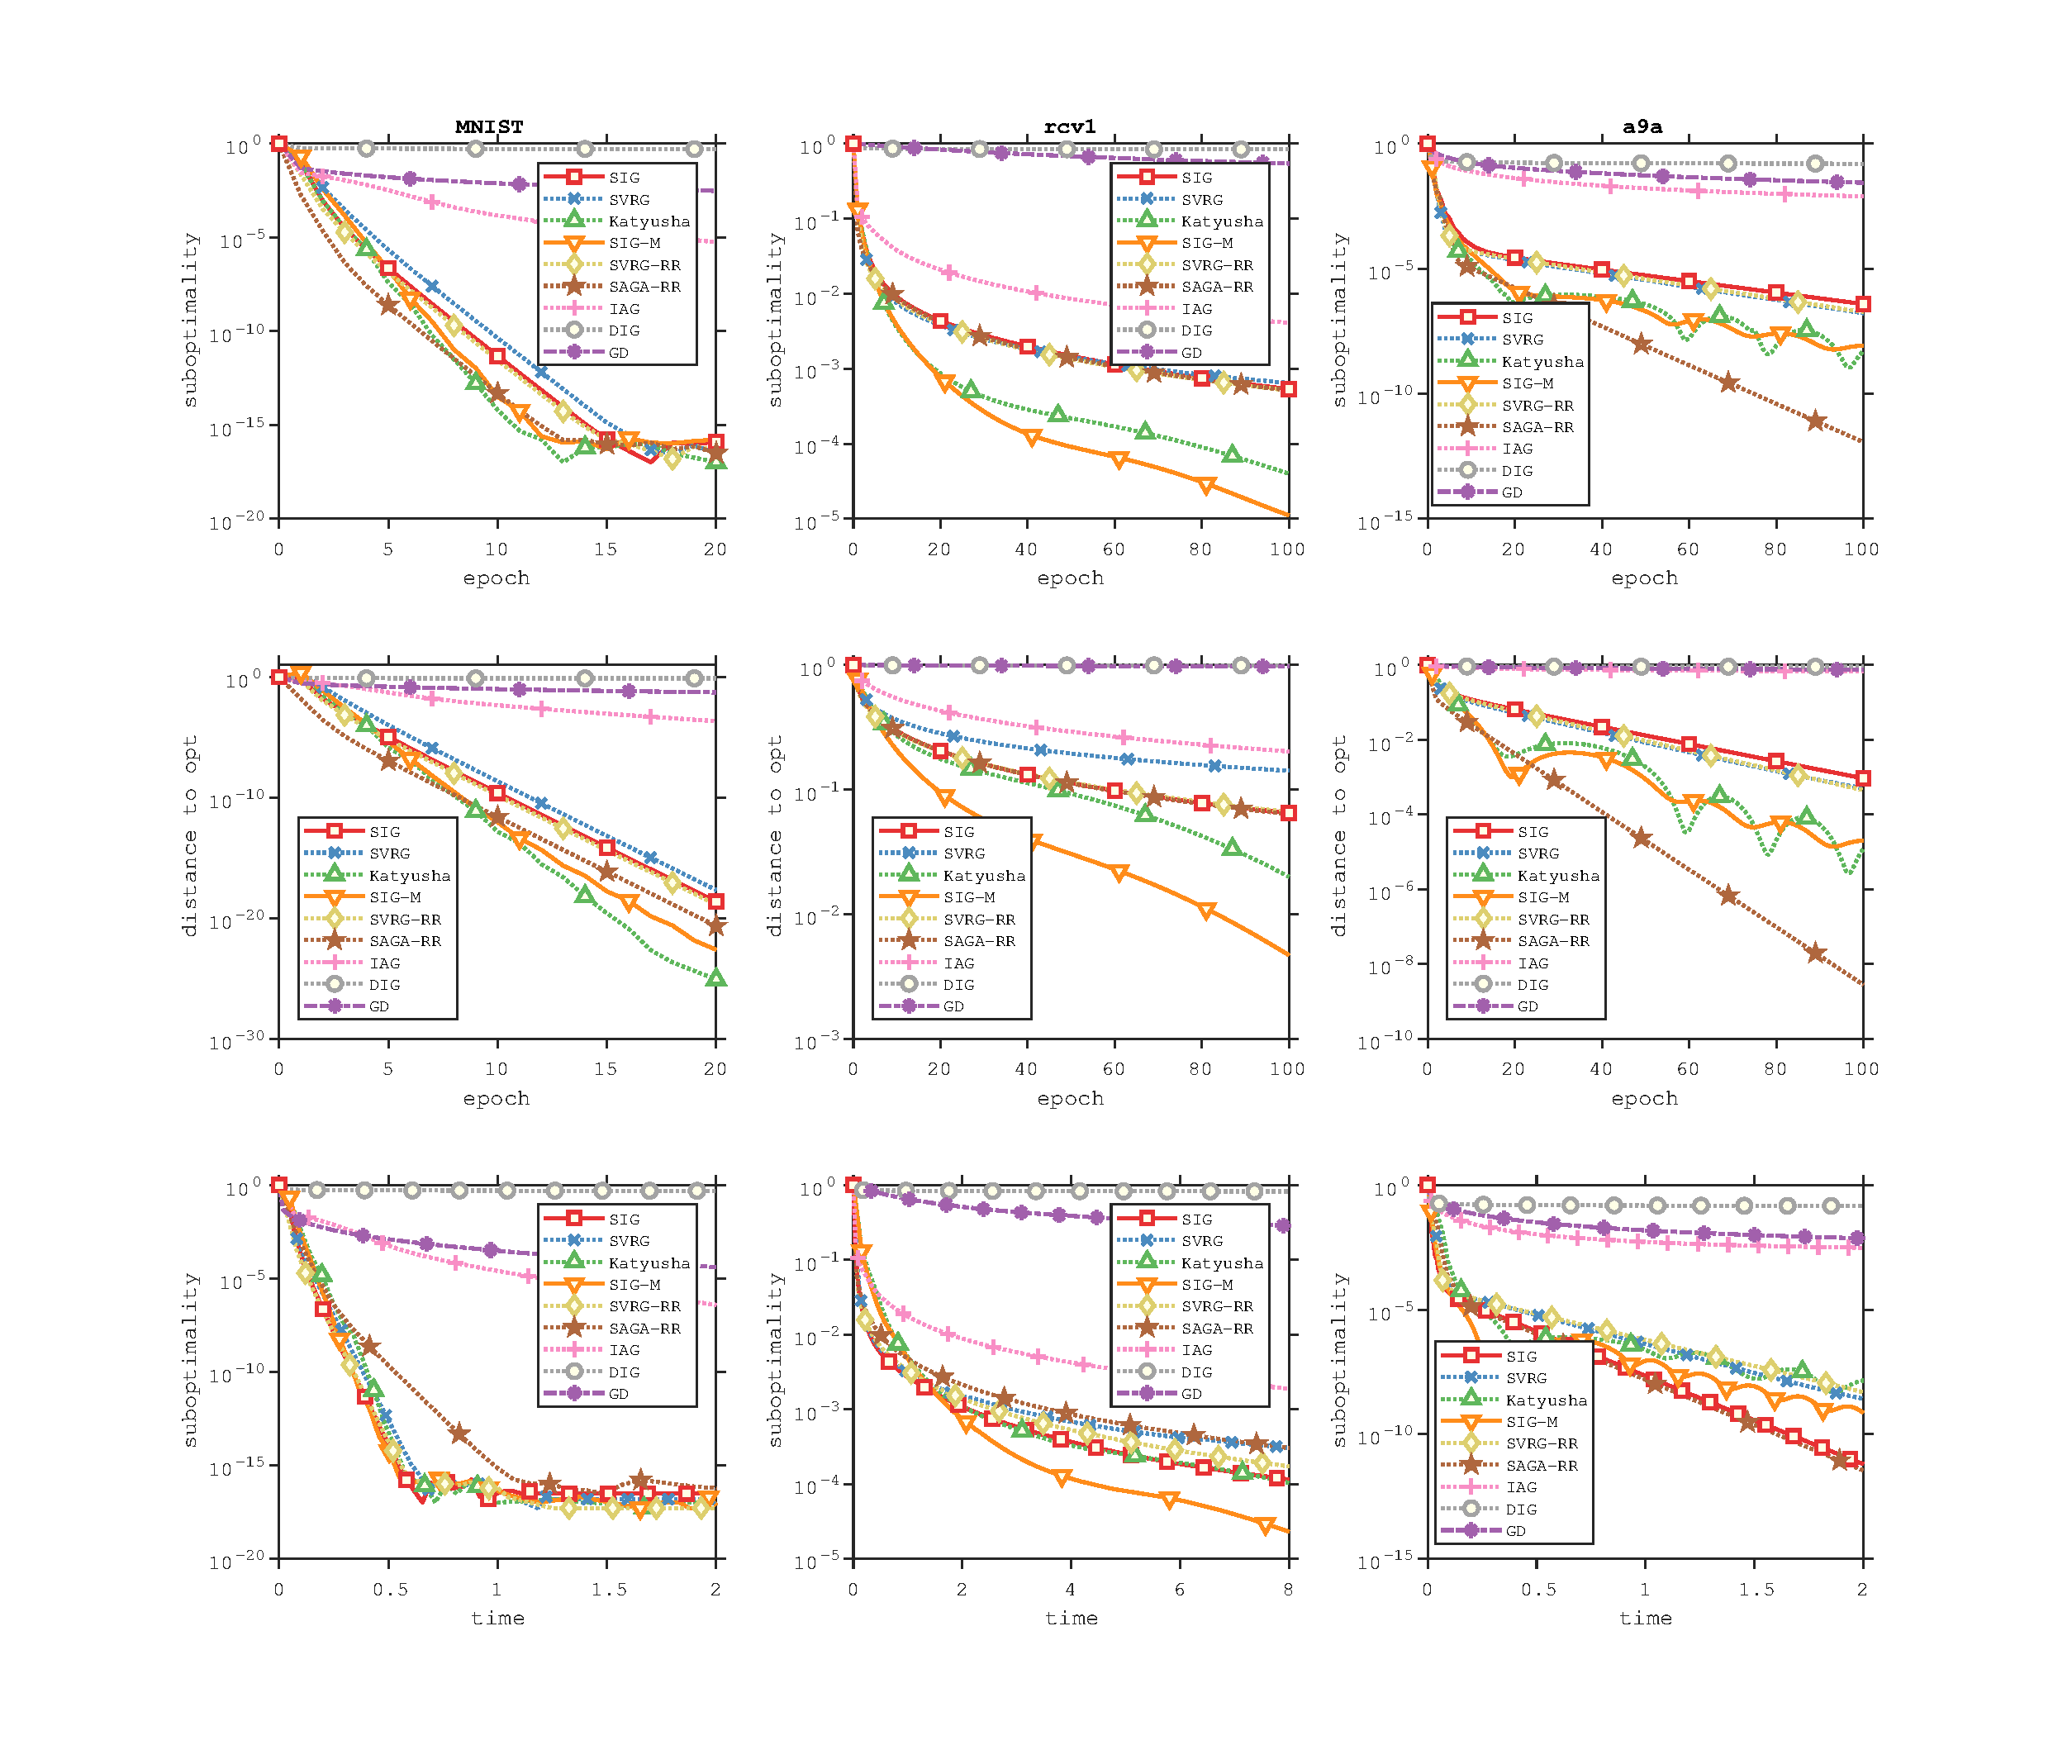
\includegraphics[trim={3.5cm 23cm 3.5cm 2cm},clip,width=11.5cm]{data/img/figure3}
            \end{figure}
        }
        \only<3>{
            \vspace*{1cm}
            \begin{itemize}
                \item 横坐标表示外循环次数
                \item 纵坐标表示迭代变量到最优解的相对距离$(\|w_0^s - w^*\|^2) / (\|w_0^0 - w^*\|^2)$
            \end{itemize}
        }
    }
    \end{overlayarea}

    \begin{overlayarea}{11.5cm}{4cm}
    {
        \only<1>{
            \begin{itemize}
                \item 横坐标表示外循环次数
                \item 纵坐标表示目标函数值的相对精度$(F(w_0^s) - F(w^*)) / (F(w_0^0) - F(w^*))$
            \end{itemize}
        }
        \only<2-3>{
            \vspace*{-0.5cm}
            \begin{figure}[H]
              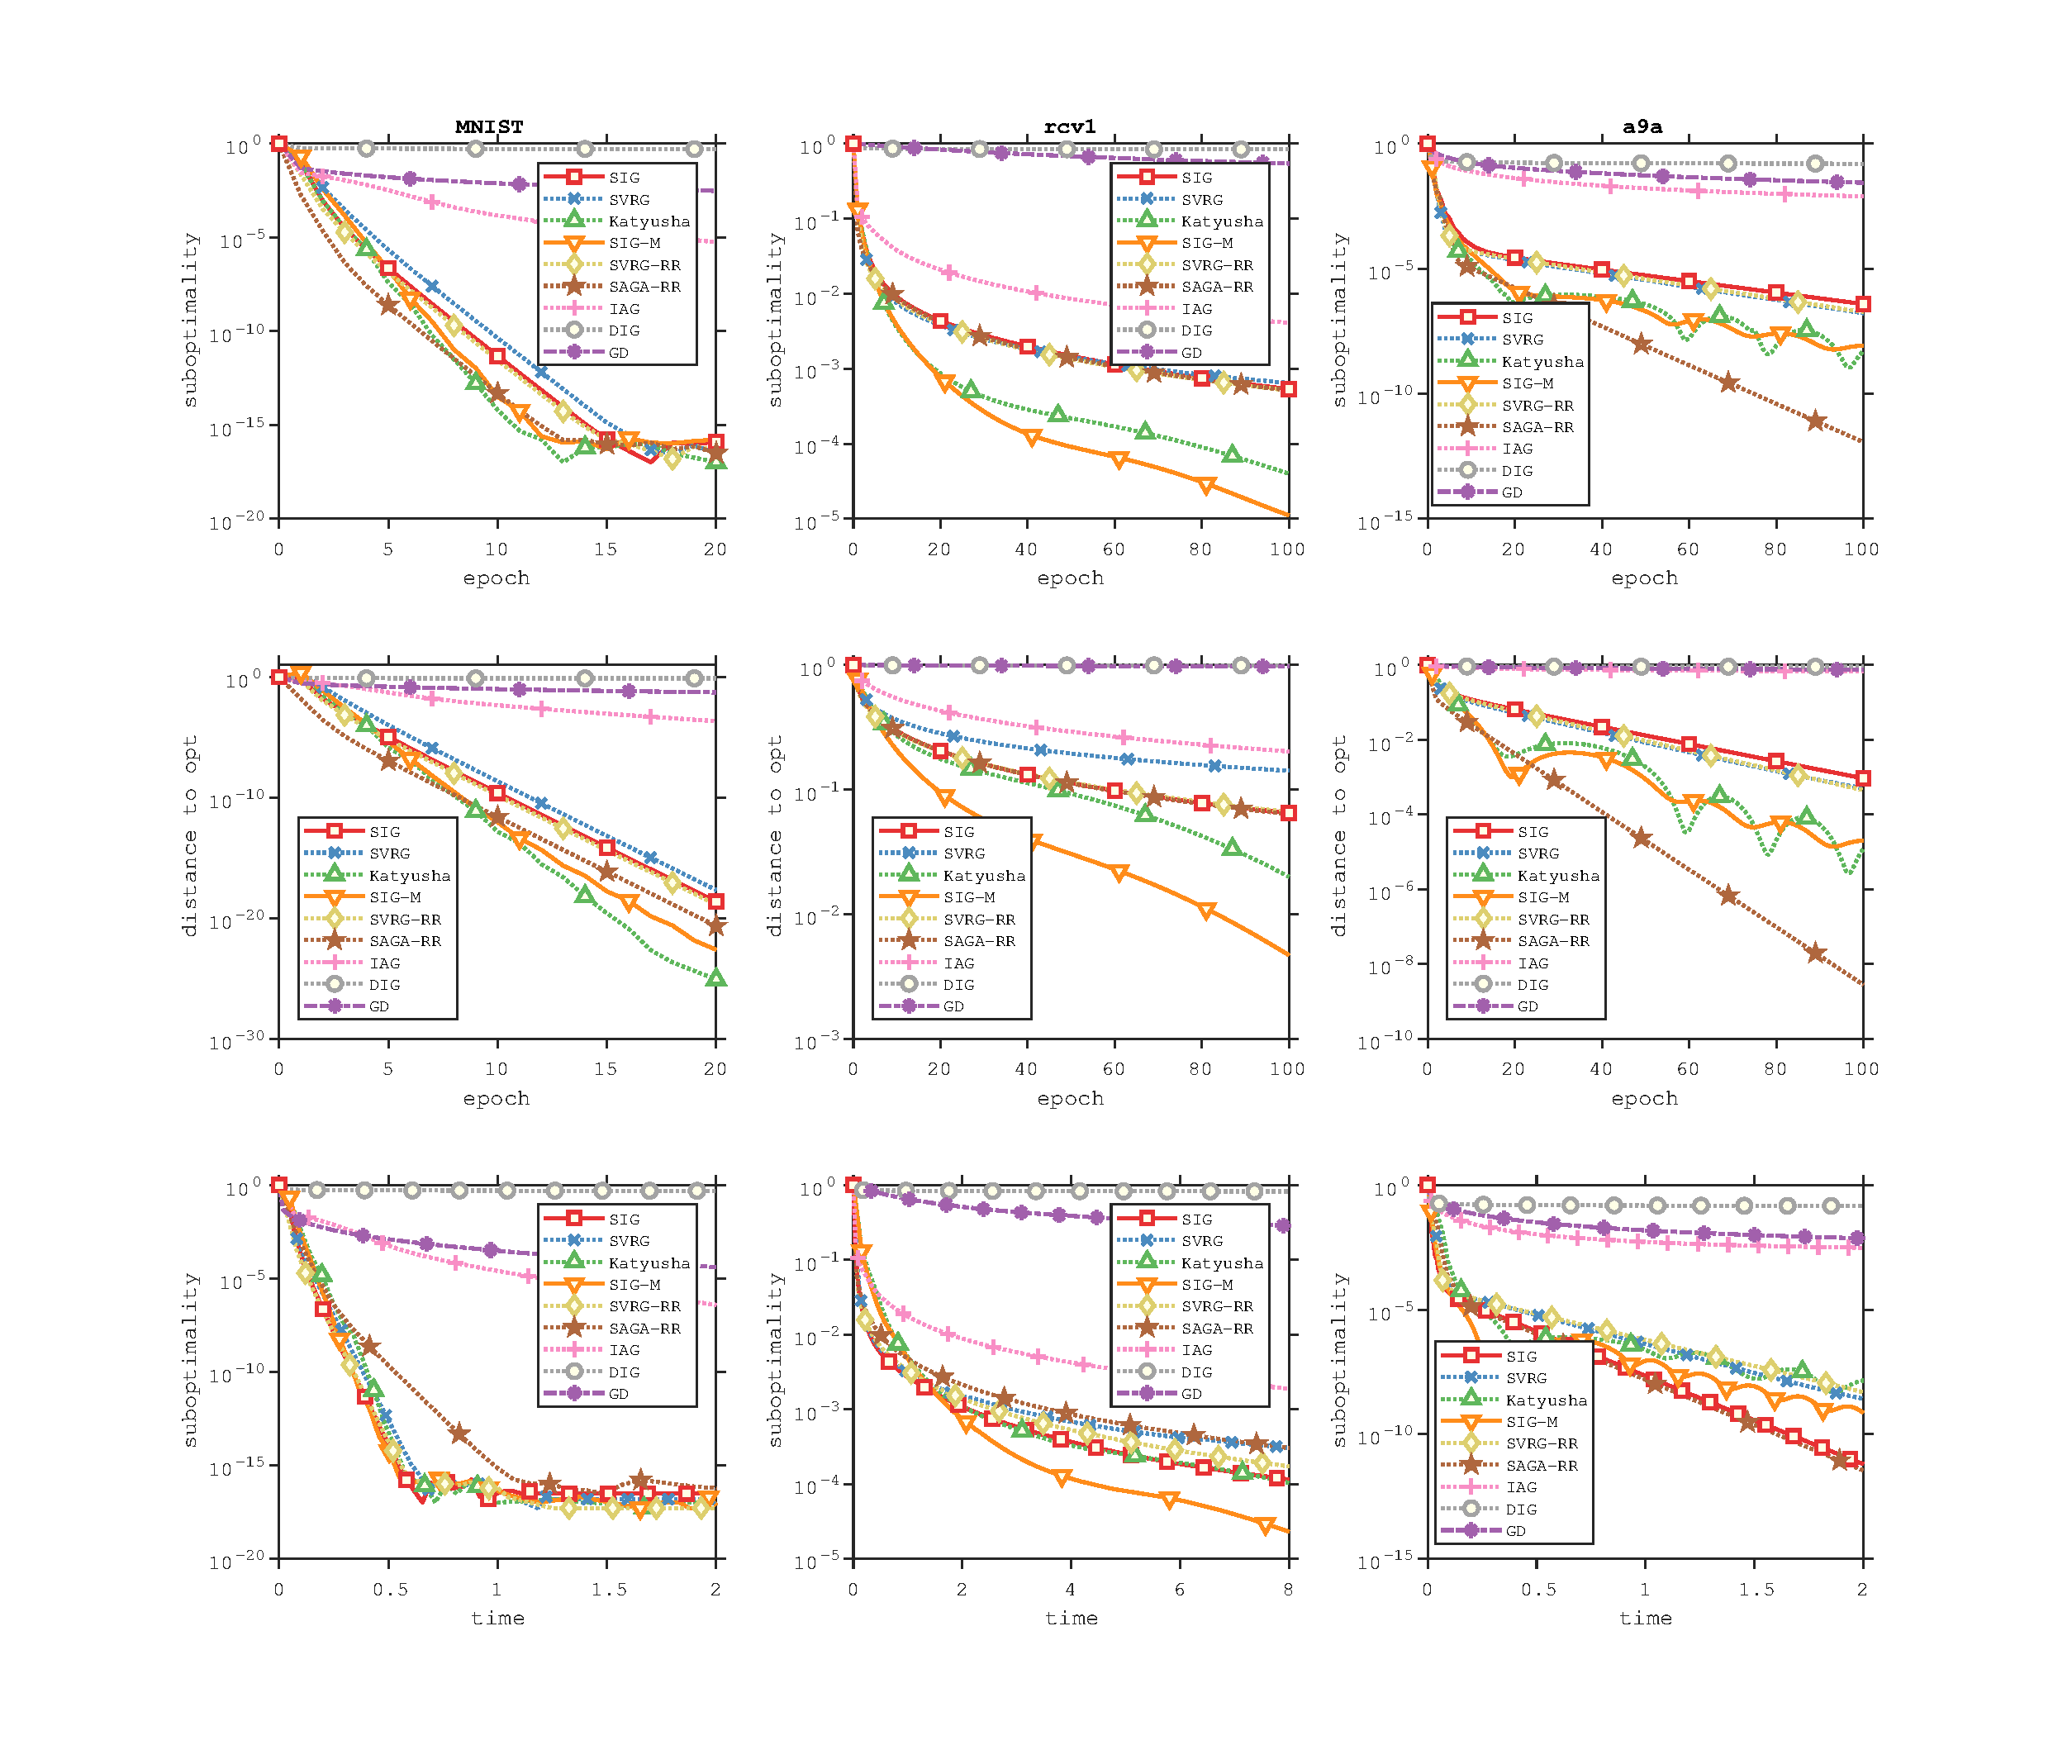
\includegraphics[trim={3.5cm 12.5cm 3.5cm 13cm},clip,width=11.5cm]{data/img/figure3}
              \caption{SIG,SIG-M及其他算法在MNIST、rcv1.binary和a9a数据集上的比较}
            \end{figure}
        }
    }
    \end{overlayarea}
  }

  \subsection{大数据集上的实验}

  \frame
  {
    \frametitle{\subsecname~ }
    \footnotesize
    \begin{itemize}
        \item 数据集:avazu,HIGGS和criteo
        \item 限制物理内存的使用上限,以模拟超大规模优化的情景
    \end{itemize}

    \begin{figure}
        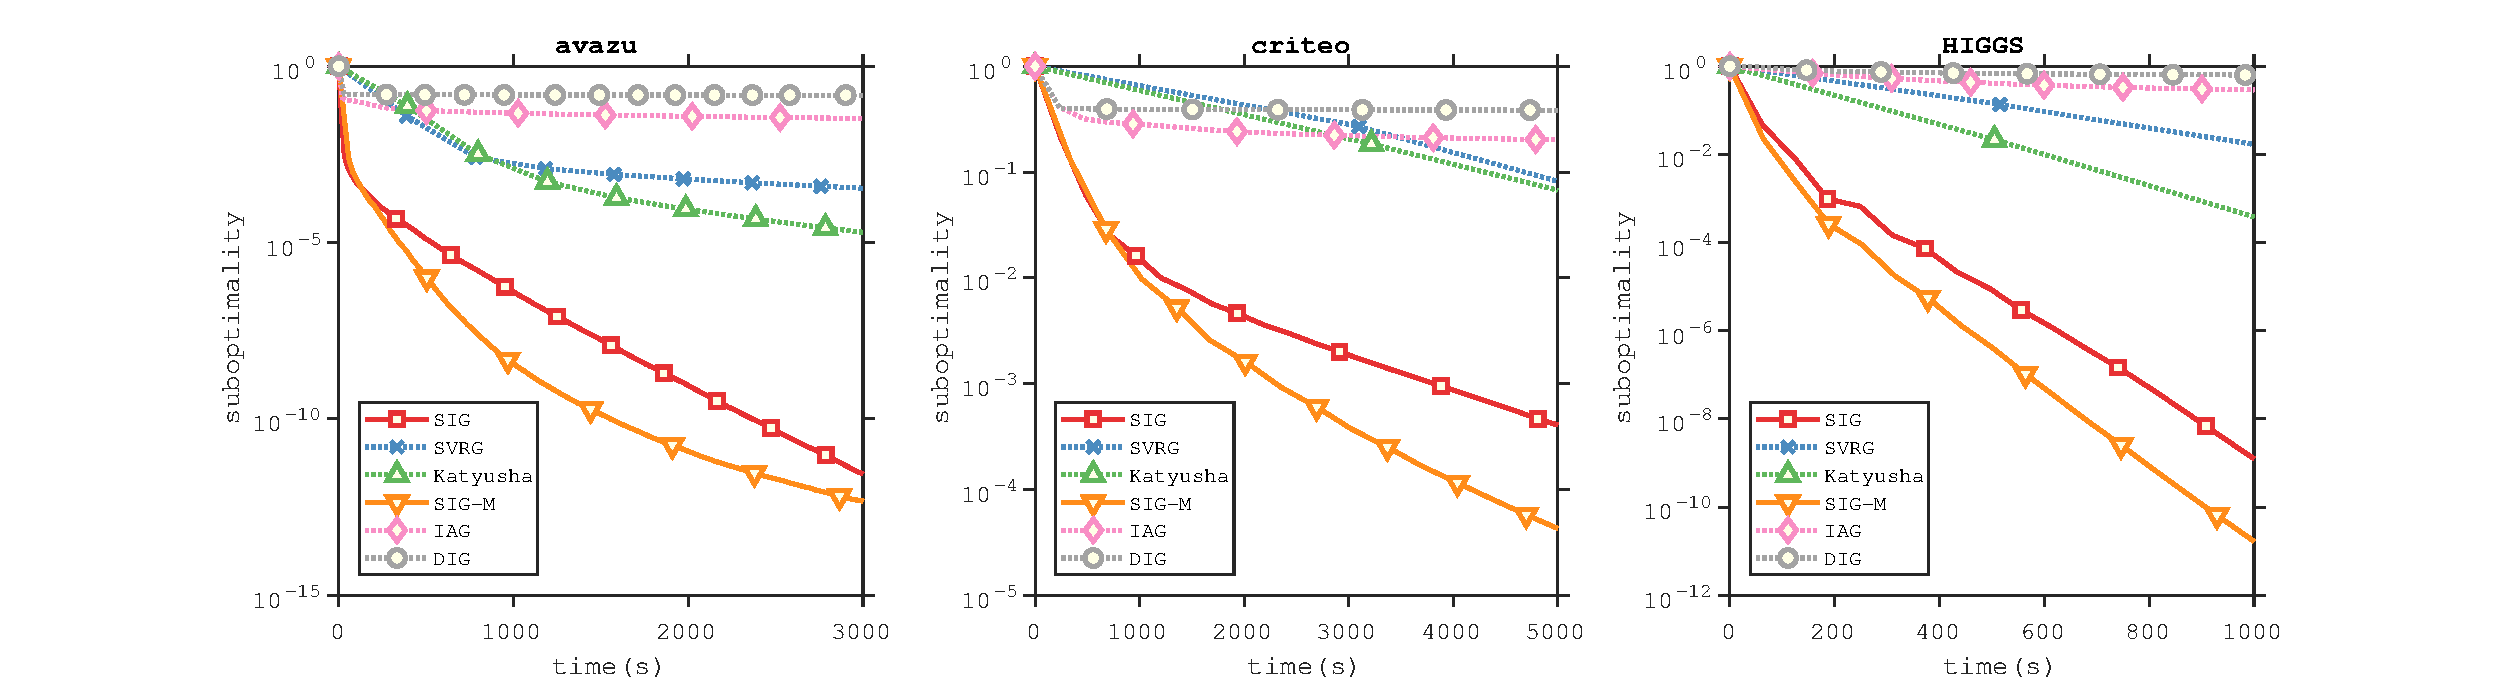
\includegraphics[trim={3.5cm 0cm 3.5cm 0cm},clip,width=11.5cm]{data/img/figure4}
        \caption{SIG,SIG-M及其他算法在avazu、criteo和HIGGS数据上的比较数据集上的比较}
    \end{figure}

  }

  \frame
  {
    \frametitle{大数据集上的实验(Cont.)}
    \footnotesize
    \begin{itemize}
        \item 比较不同的物理内存限制下SIG、SVRG的CPU时间和数据传输时间,数据集:criteo
    \end{itemize}

    \vspace*{-0.5cm}
    \begin{figure}
        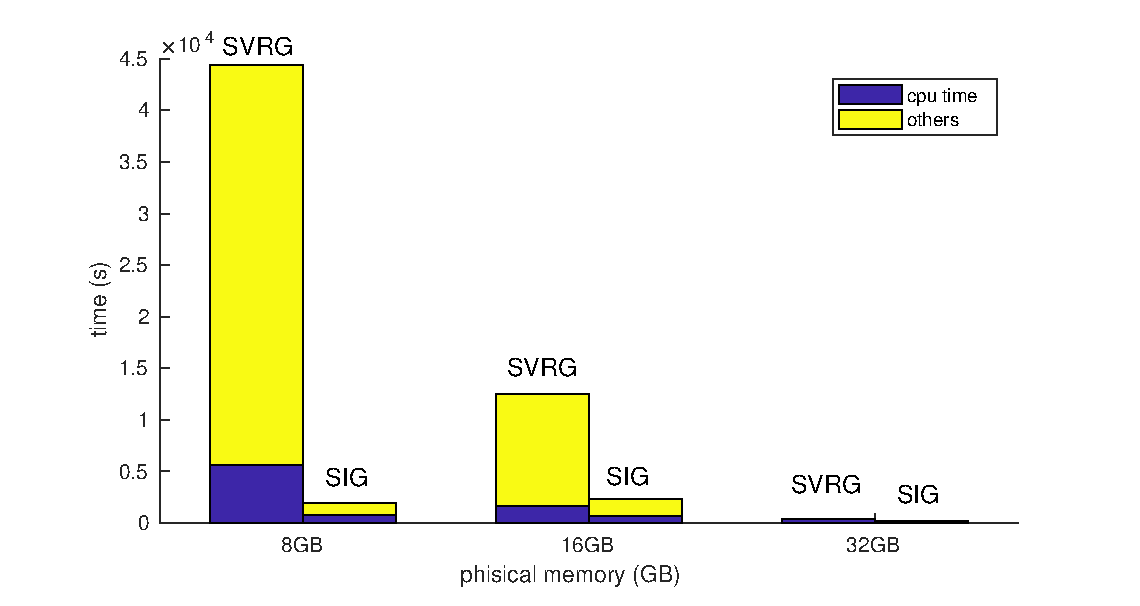
\includegraphics[trim={0 0 0 0},clip,width=11.5cm]{data/img/bar_time}
        \caption{两个算法分别运行10个外循环,横坐标表示物理内存的使用上限,纵坐标表示时间}
    \end{figure}

  }

  \frame
  {
    \frametitle{大数据集上的实验(Cont.)}
    \footnotesize
    \begin{itemize}
        \item 比较不同的物理内存限制下SIG、SVRG的收敛速度,数据集:criteo
    \end{itemize}

    \vspace*{-0.5cm}
    \begin{figure}
        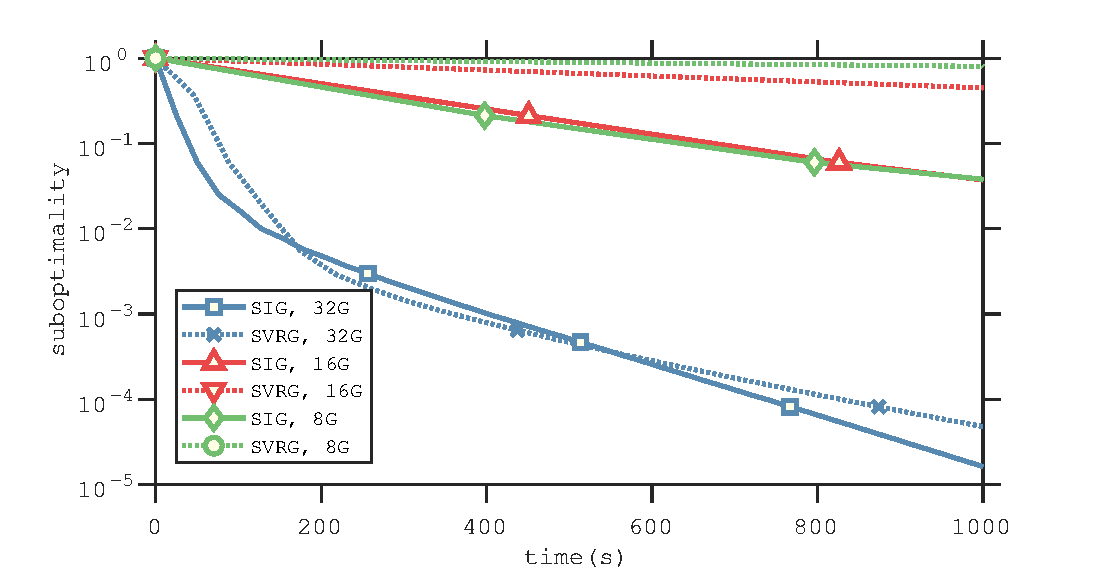
\includegraphics[trim={0cm 0 0 0cm},clip,width=0.8\textwidth]{data/img/figure6}
        \caption{SIG和SVRG在criteo数据集上、不同的物理内存限制下的收敛比较}
    \end{figure}

  }
